\subsection{Loci of Fermat and Isodynamic Equilaterals}

As seen in \cref{sec:04-brocard-isodyn-pedals}, the pedal triangles from either the Fermat $X_{13},X_{14}$ and Isodynamic $X_{15},X_{16}$ points are equilateral. Since the homothetic family conserves $\Sha=\cot\omega$, \cref{prop:04-equi-areas} implies:

\begin{corollary}
Over homothetic 3-periodics, the areas $A_k$, $k=13,14,15,16$ of the equilateral pedals from the Fermat and Isodynamic points are invariant.
\label{cor:06-equi-areas}
\end{corollary}

Over the Brocard porism, the loci of said equilaterals, were shown to be circles, see \cref{fig:04-isodynamic-equis}. Interestingly, and referring to \cref{fig:06-homot-equis}:

\begin{figure}
    \centering
    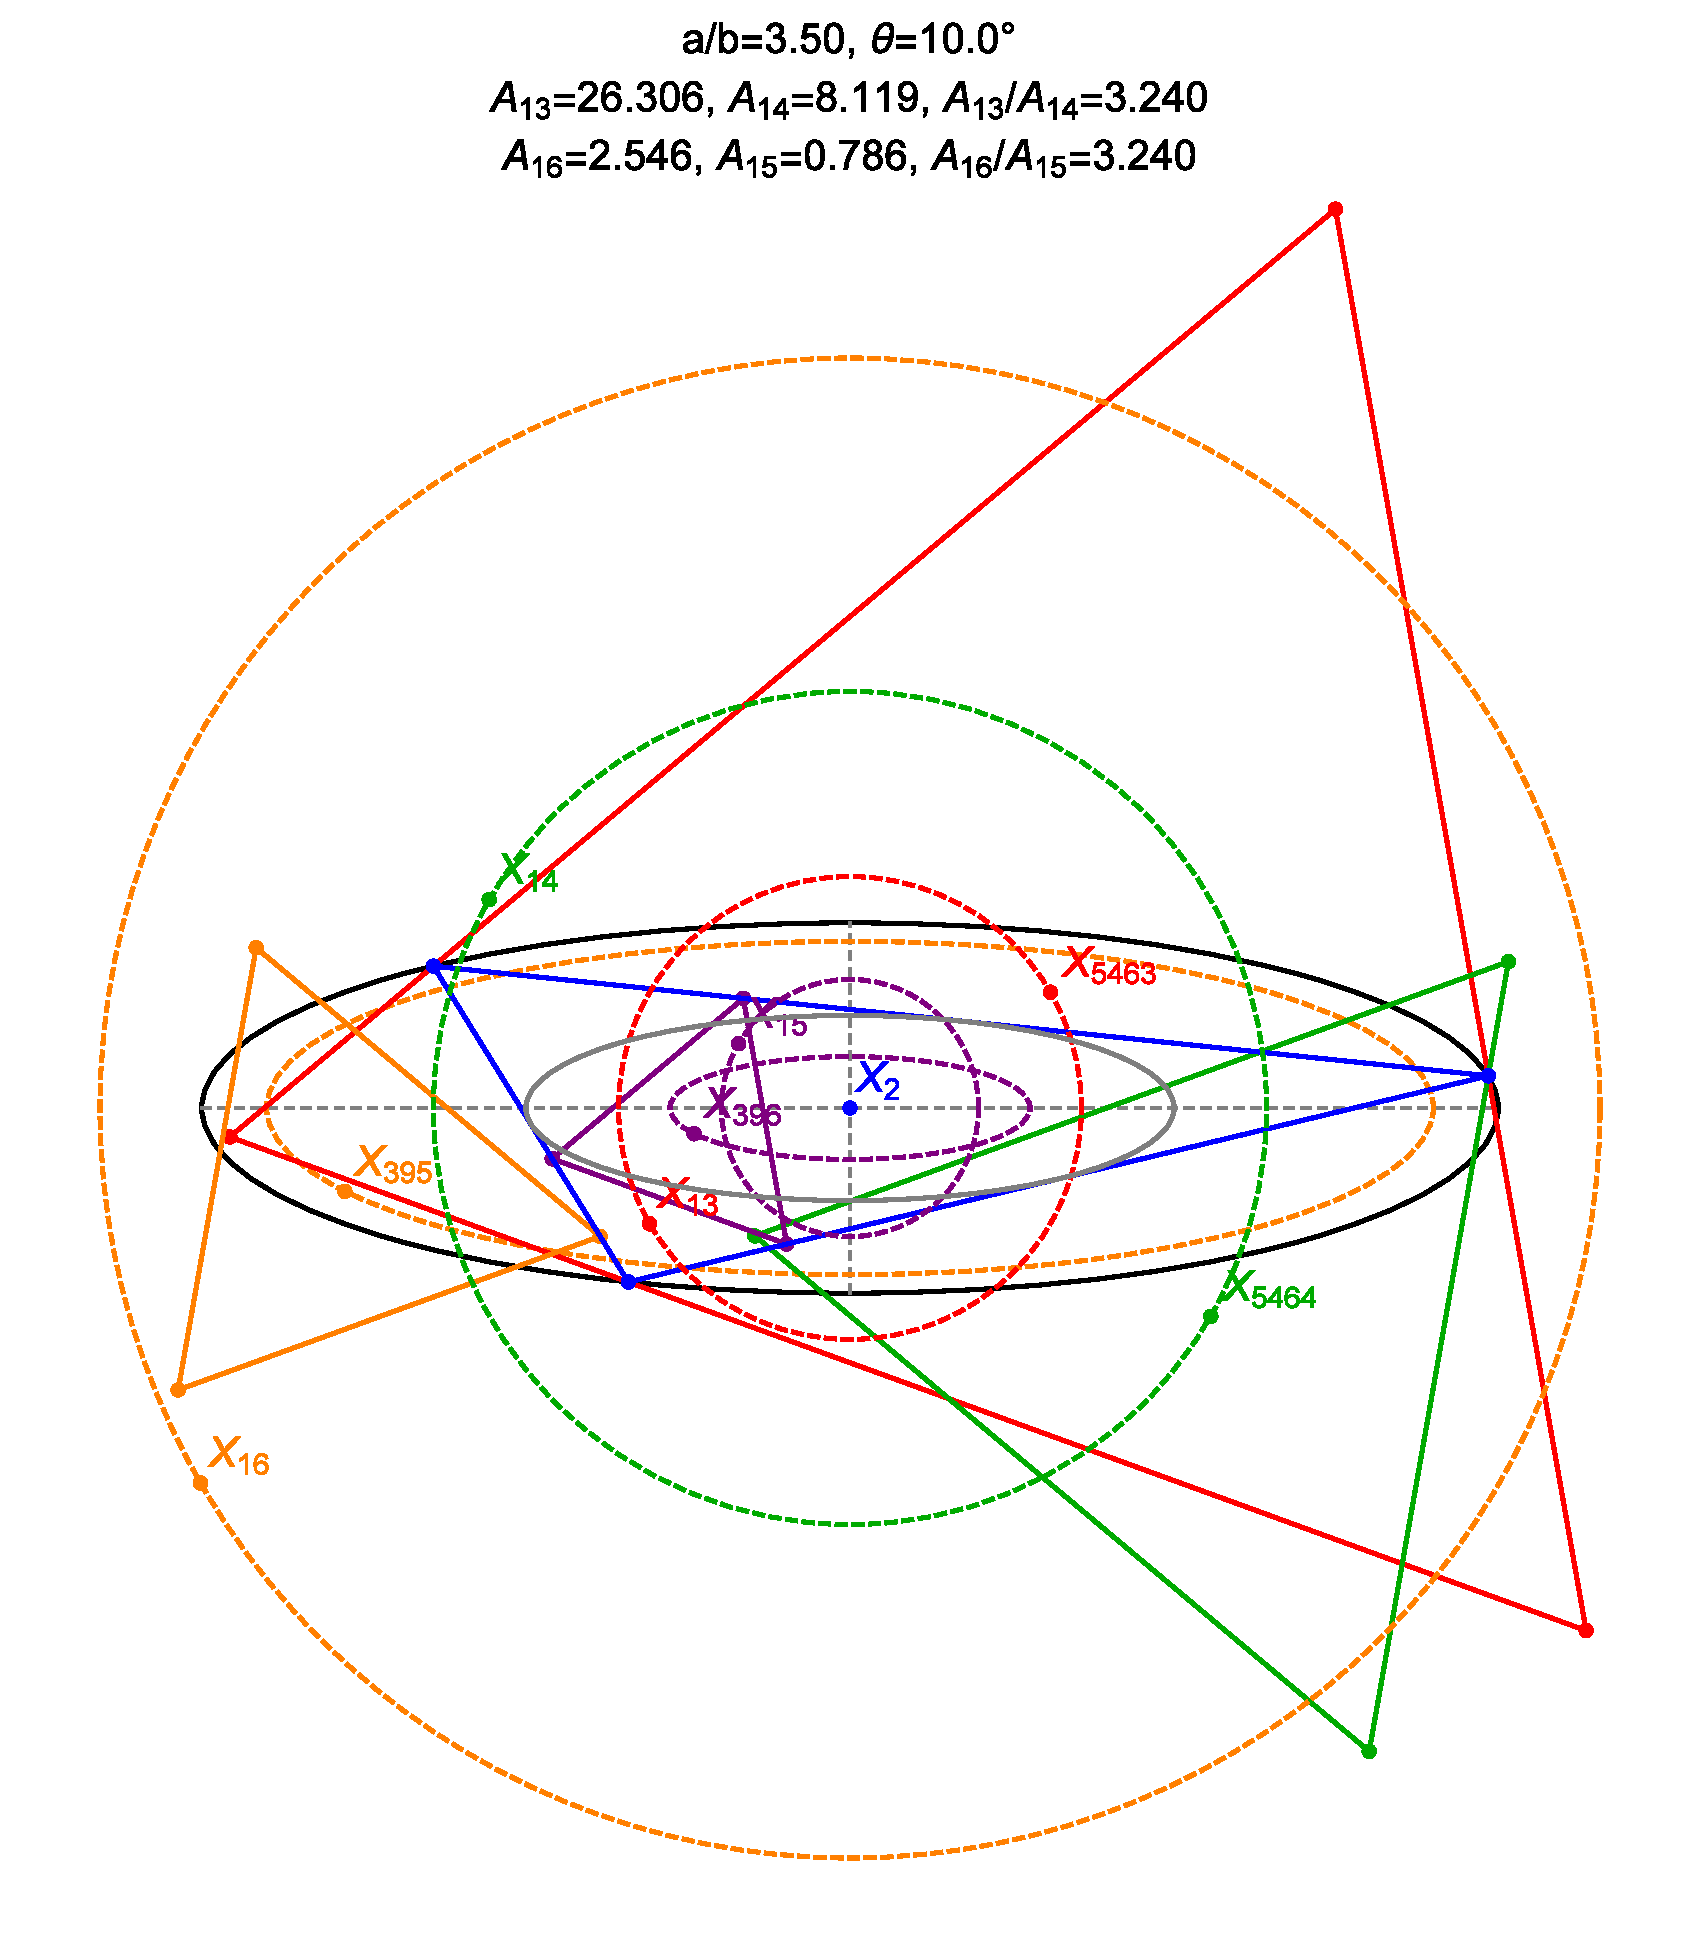
\includegraphics[width=\textwidth]{pics_06_090_homot_isos.eps}
    \caption{The homothetic Poncelet family (stationary $X_2$) is equibrocardal (conserves $\omega$) and its triangles (blue) have invariant area. The loci of $X_k,k=13,14,15,16$ are circles concentric with the ellipses \href{https://youtu.be/ZwTfwaJJitE}{Video}. Since areas $A_{15}$, $A_{16}$, $A_{13}$, $A_{14}$ only depend on $\cot\omega$, they are individually invariant. The loci of $X_{396}$ and $X_{395}$ are ellipses whereas those of $X_{5463}$ and $X_{5464}$ are circles.
    \href{https://youtu.be/7qoxAaG8sbk}{Video}}
    \label{fig:06-homot-equis}
\end{figure}